\documentclass[12pt]{report}
\usepackage[a4paper, margin=0.5in]{geometry}
\usepackage{tikz, xcolor, graphicx, wrapfig, hyperref, amsmath, amssymb, geometry, array, float, caption}
\renewcommand{\familydefault}{\sfdefault}
\usepackage[scaled]{helvet}
\usepackage[table]{xcolor}
\geometry{margin=1in}


\usepackage{titlesec, comment}

\titleformat{\chapter}[display]
  {\normalfont\huge\bfseries}{}{0pt}{\Huge\vspace{-2cm}} % you can tweak this

\titlespacing*{\chapter}{0pt}{5pt}{20pt} % left, before, after


\begin{document}

\begin{comment}
  % ====================== TITLE [commented] ========================
  \begin{center}
    % \vspace*{-1in}
    
\includegraphics[width=0.4\textwidth]{sae_aerospace.png}\\
    \vspace{1cm}
    \textbf{\LARGE AEROTHON 2025} \\
    \vspace{0.5in}
    \textbf{\Large UNCREWED AIRCRAFT SYSTEM  (UAS) \\
    DESIGN, BUILD \\ AND FLY CONTEST}\\
    \vspace{0.5cm}
    
\includegraphics[width=0.4\textwidth]{aerothon2025.png}\\
    \vspace{0.5cm}
    \Large \textbf{PHASE 1:} DESIGN REPORT \\
    \vspace{0.5cm}
    \Large \textbf{TEAM NAME:} UDSAV \\
    \Large \textbf{TEAM NUMBER: } AT2025043
    
    \vspace{0.5cm}
    
\includegraphics[width=0.3\textwidth]{gsvlogo.png}\\
    \vspace{0.5cm}
    \textbf{\Large GATI SHAKTI VISHWAVIDYALAYA} \\
    \large{Ministry of Railways, Govt. of India \\Vadodara, India - 390004}
  \end{center}
  % ======================================================
  \newpage
  \begin{figure}[h] 
    \centering
    
\includegraphics[width=1\textwidth]{certificate_faculty.jpeg}
  \end{figure}
  \newpage
\end{comment}

% starting of main document for design report
  \newgeometry{left=1in, right=0.5in, top=1in, bottom=0.5in}
  % ============ [TABLE OF CONTENTS] ================
  \tableofcontents
  \newpage
\begingroup
  \let\clearpage\relax
  \listoftables
  \vspace{1in}
  \listoffigures
\endgroup
  \newpage

  \newgeometry{left=1in, right=0.5in, top=0.5in, bottom=0.5in}
  \renewcommand{\arraystretch}{1.5}
      \rowcolors{1}{white}{blue!10}

  % ================== Introduction =================
  \chapter{Introduction}
  \section{Overview}

   In the face of natural and man-made disasters, rapid response and situational awareness are critical. Drones have emerged as powerful tools in disaster management, offering real-time aerial insights, access to hard-to-reach areas, and faster deployment compared to traditional methods. Whether locating survivors, assessing damage, or delivering essential supplies, drone technology enhances the efficiency and safety of relief operations. As disasters grow more complex and unpredictable, integrating drones into emergency response systems is no longer a luxury—it's a necessity. \\ 

   Through Aerothon, Team UDSAV (\textit{Uncrewed Disaster Surveillance Aerial Vehicle}) is not just competing—we are contributing to the evolution of drone-assisted disaster response, pushing the boundaries of what UAVs can achieve in life-saving missions.
   \begin{figure}[h]
        \centering
        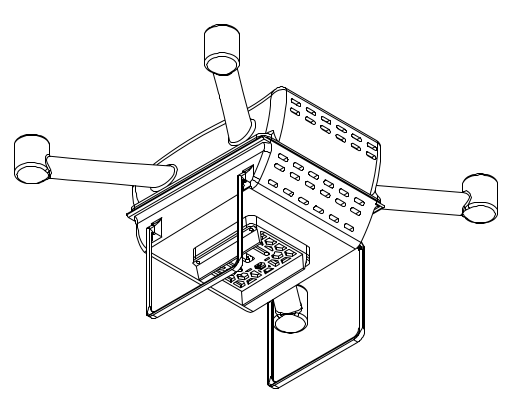
\includegraphics[width=0.5\textwidth]{droneschematic2d.png}
        \label{fig:udsav}
      \end{figure}


    \section{Problem Statement and Mission Requirements}
    This year's AEROTHON is themed on \textbf{\textit{Surveillance and Disaster Management.}} The problem statement is to build an \textbf{\textit{Uncrewed Aircraft System (UAS)}} to be able to perform the mission requirements as per the rulebook. The mission requirements at a glance are as follows: \\ \\
    \textbf{Mission - 1:} \textit{Advanced Obstacle Navigation $\&$ Fragile Payload Delivery with Precision Placement – Manual Operation} \\ \\
    \textbf{Mission - 2:} \textit{Autonomous Object Classification, Disaster Situation Identification $\&$ Payload Drop – Autonomous Operation} 



    \section{Scope of Report}
    The scope of this report is to provide a comprehensive understanding of the design rationale we have used while building this project. We have tried to provide the relevant calculations, figures, and analysis models to justify the materials/design/framework we've chosen to work with for our structural and system architectures. \\ 

    \noindent Apart from that, this report is intended to also serve as an accessible guide catering to neophytes in UAV/UAS systems. We have tried our best to aim at providing clear context and insight that sort of demystifies drone development. \\

  % ======== Requirements and Design Objectives =========
  \section{System Requirements \& Design Objectives}
    \subsection{Mission Profile}
    \begin{enumerate}
      \item \textbf{Mission 1:} \textit{Advanced Obstacle Navigation $\&$ Fragile Payload Delivery with Precision Placement} \\
        This is a \textbf{\textit{Manual Operation.}} In this mission, the drone must transport a fragile payload through a challenging course filled with static obstacles such as walls, barriers, and narrow passages. The primary objective is to navigate these obstacles with high precision while ensuring the payload remains undamaged. \\
        
        Upon reaching the target zone, the drone must land carefully and place the fragile payload on the ground without causing any damage. After the successful placement, the drone must then return to the takeoff point or designated home base, ensuring safe and efficient navigation back through the course. The mission is complete once the payload is placed securely, and the drone successfully returns to the home base.
      \item \textbf{Mission 2:} \textit{Autonomous Object Classification, Disaster Situation Identification $\&$ Payload Drop }\\
        This is an \textbf{\textit{Autonomous Operation.}} In this mission, the drone will autonomously scan, classify, and assess objects within a predefined area using onboard sensors and algorithms. The objects will vary in shape, size, color, and structure, and may be partially obscured, presenting challenges for detection and classification. Once the objects are classified, the drone will identify potential disaster scenarios, such as flooding, fire, or damaged infrastructure, within the same area.
    \end{enumerate}
    \subsection{Key Performance Indicators \& Constraints}
    According to the above defined mission profiles, we have a few KPIs (\textit{Key Performance Index}) to keep in mind.
    \begin{enumerate}
      \item Flight Endurance and Range 
      \item Payload Handling 
      \item Autonomous Capabilites
      \item System Reliability
      \item Design and Innovation
    \end{enumerate}
        The design and development of the UAV is subjected to several constraints as per the guidelines mentioned in the rulebook AEROTHON 2025. These include dimensional constraints, payload restrictions and strict autonomy requirements. The drone must perform all missions bound by these constraints and we have taken great time and care to articulate them down to ensure nothing is amiss.
    \begin{enumerate}
      \item \textbf{Dimensional Constraints}
        \begin{itemize}
          \item Maximum Wingspan: \textbf{1.5 metres} - the UAV must fit inside a \textbf{\textit{1.5m x 1.5m x 1.5m bounding box}} in assembled condition.
          \item Maximum Takeoff Weight: $ \boldsymbol{< 2kg} $ including battery and payload.
        \end{itemize}
      \item \textbf{Payload Constraints}
        \begin{itemize}
          \item Payload: One fragile payload cube of \textbf{\textit{12cm x 7cm x 7cm}} weighing \textbf{\textit{200g}}.
          \item Payload must be released within a \textbf{\textit{3m x 3m}} target zone.
        \end{itemize}
      \item \textbf{Flight Environment Constraints}
        \begin{itemize}
          \item Missions are conducted in \textbf{\textit{open outdoor airspace}}.
          \item Expect wind speeds upto \textbf{\textit{5m/s}}
        \end{itemize}
      \item \textbf{Autonomy and Mission Constraints}
        \begin{itemize}
          \item \textbf{Mission 1:} Manual flight only (no GPS or autopilot usage).
          \item \textbf{Mission 2:} Fully autonomous flight (no pilot intervention or RC use).
          \item All autonomous missions must avoid obstacles and make decisions based on \textbf{\textit{onboard computation.}}
        \end{itemize}
      \item \textbf{Power and Communication Constraints}
        \begin{itemize}
          \item Must operate on battery only
          \item No cellular or internet-based comms allowed
          \item Only 2.4 GHz or 5.8 GHz RF modules permitted
        \end{itemize}
      \item \textbf{Safety and Compliance}
        \begin{itemize}
          \item Must have a failsafe mode (e.g., return-to-home or emergency land)
          \item Must pass technical inspection before flying
          \item Compliance with DGCA drone guidelines (if relevant in test zones)
        \end{itemize}
      \item \textbf{Operational Constraints}
        \begin{itemize}
          \item The team must complete the flight within a \textbf{\textit{15-minute slot.}}
          \item Payload must be dropped in an area of \textbf{\textit{3m x 3m.}}
        \end{itemize}
    \end{enumerate}
  % ========= Conceptual Design Approach =======
  \chapter{Conceptual Design Approach}
    \section{Design Methodology}
    In design methodology, we followed structured top down system engineering approach. Our main mission is manual payload delivery and autonomous disaster surveillance. Once the mission is defined, we proceeded through the following design steps:
    \begin{itemize}
      \item Requirement Analysis: Key performance indicators (KPIs) such as payload stability, endurance and autonomy levels were associated to component-level specifications.
      \item Conceptual Design: Various design choices such as a multirotor configuration, frame, and AI-enabled onboard computation were evaluated.
      \item Component Selection: Each subsystem—propulsion, aerodynamics, structure, sensors—was chosen based on performance, power, weight, and cost.
      \item Iterative Prototyping: Using simulation and CAD modeling, we iteratively refine CG balance, and propulsion performance.
      \item Validation \& Optimization: The design is validated using CFD/FEM tools for aerodynamic , deformation , stress and structural behavior.

    \end{itemize}


    \section{Product Benchmark \& Trade-off Analysis} % why we chose this design over other 
    For optimizing performance and ensuring mission reliability, a benchmarking exercise was conducted. \\

\textbf{Benchmarked Categories:}
\begin{itemize}
  \item Frame type: H-frame, X-frame, and custom modular frames
\item Motor: Low vs high KV ratings
  \item Material: Carbon fiber vs aluminum vs ABS composites
  \item Computational Units: Raspberry Pi vs Jetson Nano/Orin for onboard processing
  \item Flight Controllers: Pixhawk vs DJI N3 vs Navio2
  
\end{itemize}

  \textbf{Trade-off Analysis:}
\begin{itemize}
  \item Each option was assessed across several key criteria:
  \item Weight vs Strength (e.g., carbon fiber offers great stiffness at low weight)
  \item Cost vs Performance (e.g., Jetson Orin offers better AI capabilities than Pi but is costlier)
  \item Thrust vs Efficiency (e.g., higher KV motors offer more speed and power)
\end{itemize}
                               
  % ======== Aerodynamic and Flight Performance ======
  \chapter{Detailed Design Breakdown}                                 
    \section{Preliminary Weight Estimation}
      \begin{table}[H]
      \centering
      \caption{Detailed Weight Breakdown}
        \begin{tabular}{|>{\raggedright\arraybackslash}p{6cm}|>{\raggedright\arraybackslash}p{6cm}|}
          \hline
          \textbf{Parameter} & \textbf{Weight \textit{(gms)}} \\
          \hline
          NVIDIA Jetson Orin Nano & 176 \\
          Pixhawk 2.4.8	& 39 \\
          Camera (\textit{x2})	 & 20 \\
          SpeedyBee BL32 50A 4-in-1 ESC	& 90 \\
          DYS D2836-7 1120KV BLDC (\textit{x4}) &	280 \\
          Battery	({\small Orange 5200mAh 11.1V
3S)} & 360  \\
          GPS – Neo M8N & 	23  \\
          \textcolor{red}{Transmitter (SkyDroid)} & 	\textcolor{red}{525} \\
          Receiver & 17 \\
          Payload	& 200 \\
          Additional Wiring & 50 \\
          Servo Motor & 10 \\
          Propellor (9") & 40 \\
          Estimated Frame Weight & 700 \\
          \hline
          \textbf{\textit{Total:}} & \textbf{2330} \\
          \hline
        \end{tabular}
      \end{table}
      \textcolor{red}{ \textbf{Note:} The transmitter is not a part of the UAS itself, so effective drone weight is \textbf{1805gms}. }
      
  % ============== Propulsion ====================
    \section{Thrust Requirement \& Propulsion System Selection}
      \subsection{Thrust Requirement}
      \begin{wrapfigure}{l}{0.3\textwidth}
        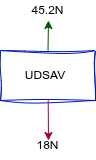
\includegraphics[width=0.175\textwidth]{thrust3.png}
        \caption{\small Thrust-to-Weight Diagram}
        \label{fig:thrustuas}
      \end{wrapfigure}
      
      To ensure stable and controlled flight, a multirotor drone must generate sufficient thrust to overcome its total weight. The drone in this design has a total takeoff weight of \textbf{1805 grams} (1.805 kg). For stable hovering, the combined thrust of all motors should ideally be at least equal to the total weight. However, to allow for effective maneuverability, rapid ascent, and compensation for wind or payload imbalance, a common design guideline is to target a thrust-to-weight ratio of at least \textbf{2:1}. This implies a minimum total thrust of approximately $2 \times 1.805 = 3.61$ kg. The selected propulsion system comprises four DYS D2836-7 1120KV brushless DC motors. According to manufacturer test data, when paired with a suitable 10$\times$4.7 propeller and a 3S (11.1V) LiPo battery, each motor can produce up to approximately \textbf{1130 grams} of thrust. Therefore, the total available thrust from all four motors is approximately \textbf{4.52 kg}, yielding a thrust-to-weight ratio of $4.52 / 1.805 \approx 2.5$. This satisfies the performance margin and confirms that the chosen motor-propeller combination is adequate for the drone's operational requirements.

      \subsection{Motor, ESC \& Propellor}
      \subsubsection{\large Motor: DYS D2836-7 1120KV Brushless Motor} 
      \begin{wrapfigure}{r}{0.3\textwidth}
        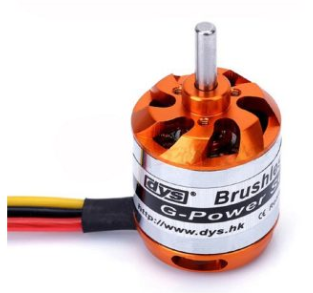
\includegraphics[width=0.3\textwidth]{bldc.png}
        \caption{DYS D2836-7 1120kV BLDC}
        \label{fig:bldc1120}
      \end{wrapfigure}
      The DYS D2836-7 1120KV Brushless Motor is our go-to motor for this project because of the following leverages it offers:
        
      \begin{itemize}
        \item \textbf{\textit{KV Rating: 1120KV}} - KV generally means RPM per volt. In layman terms, in one volt, how many rotations does it make per minute = KV. In this case, 1120KV is mid-range, which means good thrust at moderate RPMs, and it works decently with larger propellors (\textit{9" - 11"}) which improves lift and efficiency, \textit{especially} at low speeds. This is perfect for surveillance drones that require loitering and stability. A lower KV would force us to use bulky propellors, and a higher KV would drain the battery faster. 1120KV is a sweet spot between the two.
        \item \textbf{\textit{Power \& Efficiency:}} - With a 3S or 4S LiPo, this motor produces ~800g to 1100g of thrust, depending on the propeller used. It can pull 20–25A max, so it's efficient for mid-weight UAVs (\textit{in our case, it is around \textbf{1.5 ~ 2kg AUW} (All Up Weight.)}), so it's ideal for our choice.
      \end{itemize}
      
      \subsubsection{\large ESC: SpeedyBee BL32 50A 4-in-1 ESC} 
      \begin{wrapfigure}{r}{0.3\textwidth}
        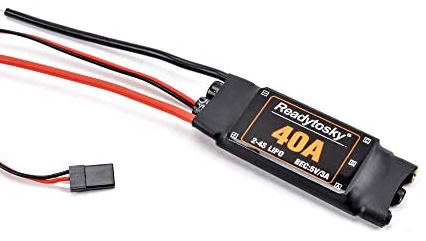
\includegraphics[width=1\linewidth]{esc.png}
        \caption{SpeedyBee BL32 50A 4-in-1 ESC}
        \label{fig:esc50a}
      \end{wrapfigure}

      The SpeedyBee BL32 50A 4-in-1 ESC is a good choice for surveillance drones, and our use case for the following reasons:
      \begin{itemize}
        \item \textbf{\textit{High Current Rating (50A per motor):}} Supports high-thrust motors and larger propellers. Useful for longer flight times, heavy payloads (cameras, sensors, gimbals), and stable cruising. Provides headroom — motors drawing 20–30A will run cooler and more reliably under a 50A ESC.
        \item \textbf{\textit{BLHeli\_32 Firmware:}} Smoother motor response, more efficient power delivery, and better low-end throttle control, which helps in steady hovering and slow maneuvering — perfect for surveillance.
        \item \textbf{\textit{4-in-1 Design:}} Combines 4 ESCs into one board, and reduces weight and wiring complexity. Makes the stack cleaner, ideal for modular or compact drone frames. Fewer potential failure points (vs. 4 individual ESCs).
        \item \textbf{\textit{Telemetry \& Monitoring:}} Supports ESC telemetry (RPM, current, temperature) via BLHeli\_32. This is important for diagnostics, health monitoring, and autonomous missions — ensuring no motor overheats or fails mid-flight.
        \item \textbf{\textit{Built for 3–6S LiPo:}} Offers flexibility across drone designs. For surveillance, a 4S or 6S setup is common due to higher efficiency and flight duration. This ESC handles both without issue.
        \item \textbf{\textit{Built-in TVS Protection:}} Has \textbf{Transient Voltage Suppression diodes} that protect against voltage spikes — vital for drone safety, especially in critical missions.
      \end{itemize}

      \subsubsection{\large Propellor: HQProp Thin Electric Prop 9×5 (2CCW) Propeller}
      \begin{wrapfigure}{r}{0.3\textwidth}
        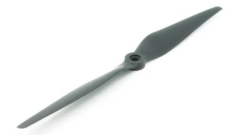
\includegraphics[width=1\linewidth]{prop.png}
        \caption{HQProp Thin Electric Prop 9×5 (2CCW) Propeller}
        \label{fig:prop9x5}
      \end{wrapfigure}

      This propeller is perfect for our use case for the following reasons:

      \begin{itemize}
        \item \textbf{\textit{High Efficiency for Long Endurance Flights:}} It is Thin electric profile = low drag → reduces current draw. Designed for cruise efficiency over brute force thrust, it serves perfect for surveillance missions where hovering and slow, steady forward flight dominate.
        \item \textbf{\textit{Optimized for Mid-Sized Motors (like D2836-7):}} The 9-inch diameter is a good disc area for smooth lift, and 5-inch pitch gives moderate speed per RPM (good forward motion without excess current). These features allows it to pair well with 1000–1200KV motors on 3S LiPo → ideal thrust-to-efficiency balance.
        \item \textbf{\textit{Smooth Throttle Response:}} Thin blades create less turbulence and vibration. This is crucial for gimbal-mounted cameras or FPV systems, reducing jello and image blur.
        \item \textbf{\textit{Expected Performance on 3S + DYS D2836-7:}} 
          \begin{enumerate}
            \item Static Thrust \hfill 850--1000g
            \item Current @ full throttle \hfill 15--18A
            \item Thrust Efficiency \hfill $\approx$ 60--65 g/W
          \end{enumerate}
      \end{itemize}
      
      \subsection{Propulsion Powertrain Efficiency}
      The total powertrain involves all the individual components that draw power from the battery, this includes things like the flight controller and flight computer. Here we are interested only in the propulsion powertrain. The propulsion powertrain typically includes: \[ \text{Battery} \quad \quad \rightarrow \quad \quad  \text{ESC} \quad \quad \rightarrow \quad \quad \text{Motors} \]

      The battery and ESC are suppliers, they supply on demand, and since all 4 motors won't derive the same amount of current (and hence power) at the same point of time-- the real-life parameters will vary in time. Here we assume that all motors demand the same power at all times.\\ \\ To quantify the overall efficiency of the UAV’s propulsion system, we analyze losses in each powertrain component. That is mathematically given by, 
      \[ 
      \boldsymbol{\eta_{total} = \eta_{battery} \times \eta_{esc} \times \eta_{motor}}
      \]

      In order to calculate each of these components, we would need to calculate the power input and output at each stage. Since we don't currently have access to each component at the moment, we're going to use the parameters provided by the manufacturers for this calculation. \\ \\
      \subsubsection{\large Battery Efficiency Derivation:}
      Given are the following from datasheets:
      \begin{itemize}
        \item Voltage (V): \hfill 11.1V
        \item Max Discharge Current: \hfill 208.0A (40C)
        \item Max Power Output ($ P_{battery} $): \hfill V x I = 11.1 x 208 = \textbf{2308.8 W}
      \end{itemize}
      This output power from the battery shall be used as input to the ESC. Now, to calculate the efficiency of battery, we can define it as, \[ \eta_{battery} = \frac{P_{out}}{P_{stored}} \] But in-flight, it's more feasible to model this using internal resistance. So, 
      \begin{gather*}
        \text{Power lost in battery} = I^2 \, R_{int} \\
        \eta_{battery} = \frac{VI - I^2 R_{int}}{VI} \,\, = \,\, 1 - \frac{IR_{int}}{V}
    \end{gather*}
    Typically, for our battery, the internal resistance is $ \boldsymbol{R_{int} = 0.015 \Omega} $

    \begin{gather*}
      \text{Power loss} = (208)^2 \times 0.015 = 648.96 \, \text{W} \\
      P_{out} = 11.1 \times 208 = 2308.8 \, \text{W} \\
      P_{stored} = 2308.8 + 648.96 = 2957.76 \, \text{W} \\ \\
      \boldsymbol{\eta_{battery}} = \frac{2308.8}{2957.76} \quad \approx \quad 78.07\, \% \quad = \boldsymbol{0.78}
    \end{gather*}
      \subsubsection{\large ESC Efficiency Calculations:}
      The following data from the datasheets:
      \begin{itemize}
        \item Max Continuous Current:	\hfill50A (per channel)
        \item Voltage Range:\hfill	3–6S LiPo (up to 25.2V)
        \item Estimated Losses:\hfill	~5–10\% (heat dissipation)
      \end{itemize}
      Since this is a 4-in-1 ESC, it shares a single power input from the battery and distributes it internally to all 4 ESC channels. The output power is given by,
      \begin{gather*} 
        P_{out} = P_{in} - P_{loss}\\
        \Rightarrow P_{out} = 2308.8 - \frac{5}{100} \times 2308.8 \\
        \therefore P_{out} \,\, \approx \,\, 2193.36 \, W \\ \\
        \Rightarrow \boldsymbol{P_{in} = 2308.8W} \quad \quad \boldsymbol{P_{out} = 2193.36W} \\ 
        \boldsymbol{\eta_{esc}} = \frac{P_{out}}{P_{in}} = \frac{2193.36}{2308.8} \quad \approx \quad \boldsymbol{0.95}
      \end{gather*}
      The total power output shared by all 4-channels of the ESC is \textbf{2193.36W}. A single channel is capable of supplying, \[ \mathrm{P_{in\_motor}} = \mathrm{P_{out\_ESC}} = \frac{2193.36}{4} = \boldsymbol{548.34 \, \text{W}} \]
  

      \subsubsection{\large Motor Efficiency Derivation:}
      The following data is given in the official datasheet:
      \begin{itemize}
        \item KV Rating: \hfill1120 RPM/V
        \item Max Power: \hfill336 W
        \item Max Current: \hfill23.2 A
        \item Voltage Range: \hfill2–4S LiPo (7.4–14.8 V)
        \item Internal Resistance:\hfill 0.070 $\Omega$
        \item Propeller:\hfill 9×5
      \end{itemize}
      The algorithm to derive the motor losses goes as follows: the efficiency is given as,
      \begin{gather*}
        \eta = \frac{\boldsymbol{P_{out}}}{\boldsymbol{P_{in}}}  \\
        \text{Electrical input power:}\quad \boldsymbol{ P_{in} = V \times I} \\
        \text{Mechanical output power:} \quad \boldsymbol{ P_{out} = T \times \omega}
      \end{gather*}
      where \textbf{\textit{V}} is voltage at which thrust is rated, \textbf{\textit{I}} is current drawn at that voltage; \textbf{\textit{T}} is torque generated by the motor (in newton-meters), and $ \boldsymbol{\omega} $ is angular velocity given by, \[ \omega = \frac{2 \pi \times \text{RPM}}{60} \] 
      The RPM without any load will be $ 1120 \times 11.1V = 12432.0 \, rpm $. But when we attach the propellers, some load will be acting agaisnt them, causing the RPM to drop by an amount. Let us assume the new RPM under load is $ \boldsymbol{RPM_{load} = 12000\, rpm} $, then the angular velocity is \[ \omega = \frac{2 \pi \times 12000}{60} \approx 1256.63 \, rad/s\]
  The theoretical torque can be calculated from the formula 
  \begin{gather*} 
    \boldsymbol{\tau = K_t \, . \, I} \\
    \text{where} \quad K_t = \frac{60}{2 \pi \, K_v} \quad and \quad I \rightarrow \text{current in amps} \,\, = \,\, 23.2 \mathrm{A} \\
    \text{now, } \quad \quad K_t = \frac{60}{2 \pi \times 1120} \quad \approx \quad 0.00852 \\ \\
    \therefore \tau = 0.00852 \times 23.2 \, \, = \, \, 0.19780 \, \text{Nm} \\ \\
    \Rightarrow \boldsymbol{ P_{out} \quad = \tau \times \omega = \quad 248.57 \, \text{W} }
  \end{gather*}
  
  Therefore, the motor efficiency is \[ \boldsymbol{\eta_{motor}} = \frac{P_{out}}{P_{in}} = \frac{248.57}{336} = 0.73979 \quad \approx \quad \boldsymbol{0.74} \] which is a pretty reasonable efficiency in real world BLDC motors. Finally, the total propulsion powertrain efficiency is given as, 
  \begin{gather*}
    \eta_{total} = \eta_{battery} \times \eta_{esc} \times \eta_{motor} \\
    \Rightarrow \boldsymbol{\eta_{total}} = 0.78 \times 0.95 \times 0.74 \quad = \quad \boldsymbol{0.55}
  \end{gather*}
  The final propulsion powertrain efficiency sums upto around 55\%, which is a reasonable value considering that some of the parameters we're assumed. Real world values will obviously vary from this.
      
     
  % ======== Aircraft Sizing ========
    \section{Aircraft Sizing}
    These are 2D schematics to ensure more precise depiction of the diagrams. 3D CAD schematics are provided in the \hyperref[chap:appendix]{\textbf{Appendix}} section.

      \subsection*{Rotor Arm}
      \subsection*{Hub}
      \noindent
      \begin{minipage}{0.48\textwidth}
          \centering
          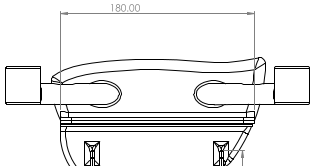
\includegraphics[width=\linewidth]{hub1.png}
          \captionof{figure}{Hub Side}
      \end{minipage}%
      \hfill
      \begin{minipage}{0.48\textwidth}
          \centering
          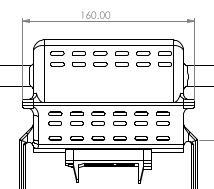
\includegraphics[width=0.7\linewidth]{hub3.png}
          \captionof{figure}{Hub Rear}
      \end{minipage}

      \vspace{1em}  % Space between rows

      % Second row: center-aligned image
      \begin{center}
      \begin{minipage}{0.5\textwidth}
          \centering
          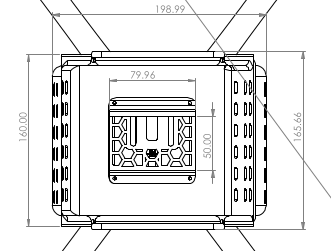
\includegraphics[width=1\linewidth]{hub2.png}
          \captionof{figure}{Hub Top}
      \end{minipage}
      \end{center}
      \subsection*{Propeller Clearance}
      
      \subsection*{Landing Gear}
      \begin{minipage}{0.4\textwidth}
        \centering
        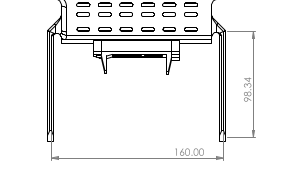
\includegraphics[width=1\textwidth]{landing1.png}
        \captionof{figure}{Rear View}
        \stepcounter{figure}

      \end{minipage}%
      \hfill
      \begin{minipage}{0.32\textwidth}
          \centering
          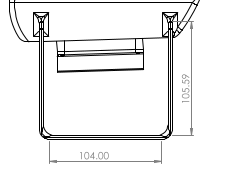
\includegraphics[width=1\textwidth]{landing2.png}
          \captionof{figure}{Side View}
      \end{minipage}%
      \subsection*{Wheelbase}
      \begin{figure}[h]
        \centering 
        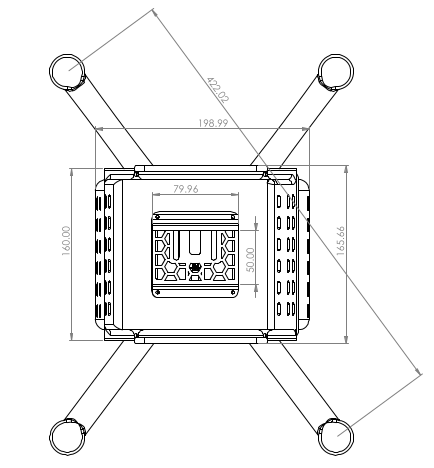
\includegraphics[width=0.5\textwidth]{wheelbase.png}
        \caption{Wheelbase = 422.02mm} 
        \label{fig:wheelbase}
      \end{figure}

      \clearpage

        
  % ======== Aircraft Performance ====
    \section{Aircraft Performance}
      \subsection{Battery Selection and Endurance}
      \subsubsection{\large Battery: Orange Pro-Range 11.1V 5200mAh (3S)} 
      \begin{wrapfigure}{r}{0.3\textwidth}
        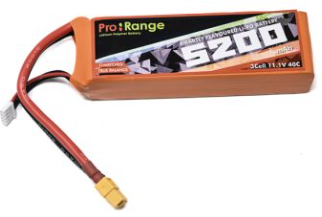
\includegraphics[width=1\linewidth]{battery.png}
        \caption{Orange 11.1V 5200mAh 3S}
        \label{fig:battery3s}
      \end{wrapfigure}
     
      The Orange Pro-Range 11.1V 5200mAh battery is the best for our use case for the following reasons: \\

      The 3S variant provides 11.1V, and has a \textbf{discharge-rate} of 40C. According to the official rated specifications, the maximum continuous discharge current is \textbf{208.0A} (\textit{40C}). It also has a max. burst discharge of \textbf{416.0A} (\textit{80C}). Let us assume that each motor draws 24A current at full-throttle, total current draw would be $ \boldsymbol{24 \times 4 = 96A} $ then \vspace{0.5cm} \[ \text{Theoretical Flight Time (hrs)} = \frac{\text{Capacity (Ah)}}{\text{Current Draw (A)}} = \frac{5.2}{96} \approx 0.0542 hrs = 3.25 mins \] But in real world applications, we dont use 100\% of the battery, we use about 60\%, so that would make the flight time around 5.2mins. 
          
      \subsection{Total Power Budget Summary}
      This sub-section summarizes the total electrical power budget of the UAS, highlighting how power from the battery is allocated to propulsion and non-propulsion (avionics and payload) subsystems.
      \begin{table}[h!]
        \centering
        \caption{Power Distribution Summary}
        \begin{tabular}{|l|p{5.5cm}|c|c|}
          \hline
          \textbf{Subsystem} & \textbf{Included Components} & \textbf{Power Demand (W)} & \textbf{\% of Total Power} \\
          \hline
          Propulsion & {\small 4 x Motors} & 1344 W & 58.2\% \\
          Avionics & {\small Flight Controller, GPS Module, Sensors (IMU, barometer)} & 6.9486 W & 0.3009 \% \\
          Communication & {\small RC Receiver, Wifi Modules}  & 20.41 W & 0.884 \% \\
          Payload & {\small 2 x Cameras} & 3.879 W & 0.168 \% \\
          Onboard Computer  & {\small NVIDIA Jetson Orin Nano 8GB Module} & 6.997 W & 0.303 \% \\
          \hline
        \end{tabular}
      \end{table}

        \subsubsection{\large Propulsion Demand}
        Based on the datasheet specification and text results, the propulsion subsystems (\textbf{\textit{4xMotors}}) demands \textbf{1344W} during peak operation. This forms the largest share of the total Power requirement ($ \sim $ 58.2 \%).
        \subsubsection{Avionics Demand}
        The avionics system forms the central nervous system of any unmanned aerial vehicle (UAV), including those designed for \textbf{Aerothon-class missions}. Its architecture and power requirements play a decisive role in shaping the overall energy distribution and electrical resilience of the aircraft. The avionics suite typically comprises a flight controller (e.g., Pixhawk), GPS module, telemetry and communication transceivers, RC receiver, and sensor systems such as IMUs and barometers. \\ 

        In advanced UAV configurations—such as ours—it is further augmented by an onboard companion computer, namely the NVIDIA Jetson Orin Nano 8GB, which performs real-time perception and decision-making tasks. \\ 

        Based on our subsystem-level analysis, the avionics block—comprising flight control, communication, and onboard computing—demands a cumulative peak power of approximately \textbf{34.36 W}. This includes:
        \begin{itemize}
          \item \textbf{6.948 W} for the flight controller and embedded sensor suite
          \item \textbf{20.41 W} for communication subsystems including RC receivers and WiFi modules,
          \item \textbf{6.997 W} for the Jetson Orin Nano, which manages AI workloads and perception.
        \end{itemize}
        While this represents only \textbf{1.49 \%} of the total system power draw, the avionics demand is non-negotiable and continuous, requiring high uptime and precision. Power is supplied via a regulated DC bus derived from the main propulsion battery, with dedicated buck converters providing clean and stable 5V and 3.3V rails to sensitive electronics.

        \subsubsection{\large Margins, Safety Factors}
        \textbf{\large Power Budget Margin:} \\
        \begin{enumerate}
          \item \textbf{Purpose:} To ensure that the chosen power source (battery) and propulsion system can consistently provide sufficient power, even under demanding conditions or if components don't perform exactly to spec.
          \item \textbf{Typical Range:} 15\% - 30\% of the calculated total power demand.
          \item \textbf{Application:} After calculating the power required for propulsion (hover, cruise, max thrust) and avionics, an additional percentage is added. 
            \[ \text{Total Required Power = (Propulsion Power + Avionics Power) * (1 + Power Margin)} \]
          \item \textbf{Considerations:} 
            \begin{itemize}
              \item Battery degradation over time.
              \item Variation in motor/propeller efficiency.
              \item Ambient temperature effects on battery performance.
              \item Increased power draw due to wind or aggressive maneuvers.
            \end{itemize}
        \end{enumerate}

        \noindent \textbf{\large Weight/Payload Margin:} \\
        \begin{enumerate}
          \item \textbf{Purpose:} To allow for small increases in component weight during design evolution, manufacturing variations, or for potential future upgrades/additional payloads.
          \item \textbf{Typical Range:} 10\% - 20\% of the estimated total weight (Empty Weight + Max Payload).
          \item \textbf{Application:} When defining the Maximum Take-Off Weight (MTOW), a buffer is included. This also impacts thrust-to-weight ratio calculations. \[ \text{Max All-Up Weight (MAUW) = (Estimated Empty Weight + Max Payload) * (1 + Weight Margin)} \]
          \item \textbf{Considerations:}
            \begin{itemize}
              \item Small design changes or additions.
              \item Manufacturing tolerances.
              \item Unforeseen weight of cabling, fasteners, etc.
            \end{itemize}
        \end{enumerate}
        \noindent \textbf{\large Battery-Capacity/Flight-Time Margin:} \\
        \begin{enumerate}
          \item \textbf{Purpose:} To ensure sufficient energy is available for the planned mission duration, plus a reserve for unexpected events (e.g., strong headwind, holding pattern, emergency landing).
          \item \textbf{Typical Range:} 15\% - 25\% of the total mission energy requirement.
          \item \textbf{Application:} After calculating the energy needed for the mission profile, additional capacity is added. Also, a "return to home" or "emergency landing" battery percentage is typically set (e.g., 20-30\% remaining). 
            \[ (\text{Battery-Capacity})_{\text{Total}} = \frac{ \text{Mission Energy Requirement} }{ \text{Battery Discharge Efficiency} } \times (1 * \text{Capacity Margin}) \] 
          \item \textbf{Considerations:}
            \begin{itemize}
              \item Battery performance degradation over cycles and temperature.
              \item Unexpected mission deviations.
              \item Wind conditions requiring higher power.
              \item Maintaining a safe reserve for landing.
            \end{itemize}
        \end{enumerate}
        \noindent \textbf{\large Structural/Safety Margin:} \\
        \begin{enumerate}
          \item \textbf{Purpose:} To ensure that the drone's airframe and structural components can withstand expected and unexpected loads without failure.
          \item \textbf{Ultimate Factor of Safety (FoS):} 1.5 - 2.0 (or higher for critical components). This is the ratio of ultimate load capacity to the maximum expected operating load.
          \item \textbf{Yield Factor of Safety:} 1.1 - 1.25. This is the ratio of yield strength to the maximum expected operating load, ensuring no permanent deformation.
          \item \textbf{Application:} Applied to material strength calculations for frame arms, motor mounts, landing gear, etc. \[ \text{Required Strength = Maximum Expected Load * Factor of Safety} \]
          \item \textbf{Considerations:}
            \begin{itemize}
              \item Dynamic loads during flight (acceleration, turns).
              \item Impact loads during hard landings or minor crashes.
              \item Vibration fatigue.
              \item Material imperfections and manufacturing variability.
            \end{itemize}
        \end{enumerate}

        

  %========== Material Selection ========
    \section{Material Selection}
      \subsection{Structural Frame, Airframe Components}
    

  %========= Ground Control
    \section{Avionics Subsystems Selection}
      \subsection{Detailed Component Breakdown}
        \subsubsection{\large Flight Controller (Pixhawk 2.4.8)}
        \begin{wrapfigure}{r}{0.3\textwidth}
          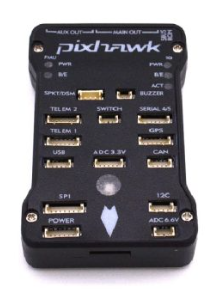
\includegraphics[width=1\linewidth]{pixhawk.png}
          \caption{Pixhawk 2.4.8}
          \label{fig:pixhawk}
        \end{wrapfigure}
        Pixhawk is widely egarded as one of the best flight controllers for drone and autonomous aircraft projects — especially in academic and research-grade prototypes — for several compelling reasons:
      \begin{itemize}
        \item \textbf{\textit{Open-Source and Flexible:}} It is built on open hardware and supported by powerful open-source firmware like PX4 or ArduPilot. This enables deep customization, ideal for research and control system testing. And for this reason also, we have \textbf{ample documentation backed by a strong collaborative community, forums, and tutorials}.
        \item \textbf{\textit{Rich I/O capabilities:}} Multiple UART, I2C, CAN, and PWM ports for connecting sensors (GPS, IMU, barometer, etc.) and actuators (ESCs, servos). Ideal for integration with multiple onboard systems including companion computers (e.g., Jetson Nano).
        \item \textbf{\textit{Compatible with autonomous and GPS-guided missions:}}  Supports autonomous navigation, geofencing, waypoints, and RTL (Return to Launch).
        \item \textbf{\textit{Built-in failsafes and safety features:}} Battery failsafes, signal loss handling, and software watchdogs protect the aircraft during unexpected conditions.
        \item \textbf{\textit{Excellent simulation support:}} Compatible with \textbf{HITL (Hardware-in-the-loop)} and \textbf{SITL (Software-in-the-loop)} for control testing and simulation.
      \end{itemize}
      
      \subsubsection{\large Flight Computer (NVIDIA Jetson Orin Nano 8GB)}
      The NVIDIA Jetson Orin Nano 8GB is a powerful, compact AI computing module designed for edge AI applications that demand both high performance and energy efficiency. In the context of our Aerothon UAV project, the Orin Nano plays a pivotal role in enabling advanced onboard computation, particularly for tasks such as \textbf{real-time image processing, autonomous navigation, and object detection.} \\

      \begin{figure}[H]
        \centering 
        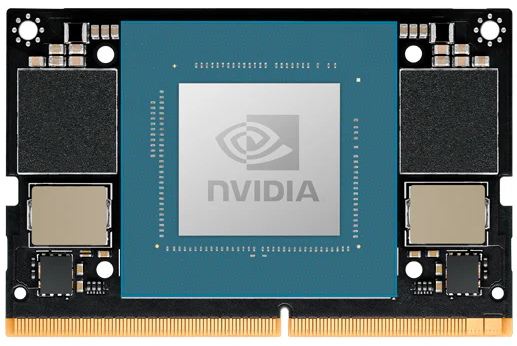
\includegraphics[width=0.5\textwidth]{jetson.png}
        \caption{NVIDIA Jetson Orin Nano 8GB Module}
        \label{fig:jetson}
      \end{figure}

      We selected this module not only for its impressive up to \textbf{40 TOPS} of AI performance but also for its \textbf{low power footprint}, which makes it ideal for flight-based applications where every gram and watt matter. The 8GB RAM ensures sufficient memory for running heavy models, such as convolutional neural networks for visual recognition or SLAM algorithms for path planning. \\

      The Jetson Orin Nano interfaces seamlessly with the Pixhawk flight controller via UART or serial USB connections, enabling a tight coupling between autonomous decision-making and low-level control. For example, live video feed from an \textbf{ESP32-CAM} or other camera modules is processed onboard the Jetson, where the output — such as target coordinates or navigation commands — is relayed to the Pixhawk for actuation. \\

      This configuration allows the aircraft to function \textbf{autonomously even without constant ground station communication}, which is critical in GPS-denied or communication-constrained environments. By offloading high-level intelligence to the Jetson module, we achieve a modular and scalable architecture that separates perception and decision-making from flight stabilization, thereby improving system robustness and flexibility. \\

      In essence, the NVIDIA Jetson Orin Nano 8GB empowers our drone with a true edge-AI brain — transforming it from a remotely controlled vehicle into a \textbf{fully autonomous aerial system} capable of intelligent flight and mission execution.

      \subsubsection{\large Cameras}
Features a 2.1mm lens with a wide FOV (up to 165°), giving the pilot a broad visual perspective, which enhances situational awareness and spatial navigation.

      We're using two different cameras, for two different purposes:
      \begin{enumerate}
          \item \textbf{FPV:} Caddx Ant Lite Analog Camera (FPV Cycle Edition) (4:3)
          \item \textbf{Object Detection:} Official Raspberry Pi Camera V2
      \end{enumerate}

      \noindent They will be placed in the drone as follows: 
      \begin{itemize}
        \item In this project, the Caddx Ant Lite serves as a live FPV feed camera transmitting real-time visuals to the ground control station.
        \item The \textbf{Raspberry Pi Camera V2} handles object detection tasks. This will be deployed on the belly of the UAV. This will provide as a guide to the gripper mechanism as well. 
      \end{itemize}

      \newpage
      \noindent \textbf{\large Official Raspberry Pi Camera V2} \\
      \begin{wrapfigure}{r}{0.3\textwidth}
          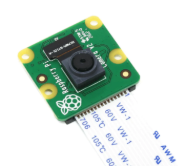
\includegraphics[width=1\linewidth]{rpicam.png}
          \caption{Raspberry Pi Cam V2}
          \label{fig:rpicam}
        \end{wrapfigure}

        We have chosen this camera for the following reasons:
        \begin{itemize}
          \item \textbf{\textit{8 Megapixel Sony IMX219 Sensor:}} Offers high-resolution image capture (3280 x 2464), which ensures that our object detection models get detailed input — especially helpful for detecting small or distant objects. 
          \item \textbf{\textit{1080p30 / 720p60 / 640x480p90 Video Modes:}} High frame rates allow for real-time object detection, essential in robotics, drones, and surveillance applications.
          \item \textbf{\textit{Low Latency Capture:}} Minimal delay in capturing frames means your detection pipeline stays fast and reactive, especially when combined with hardware acceleration (like OpenCV + TensorRT on Jetson).
          \item \textbf{\textit{Adjustable Focus (via lens mods or add-ons):}} Although the lens is fixed-focus out of the box, third-party adjustable lenses can be easily added for more precise depth-aware detection.
          \item \textbf{\textit{CSI Interface for Direct Connection:}} Connects via the CSI-2 interface (Camera Serial Interface), which provides higher bandwidth and lower CPU usage compared to USB webcams — ideal for high-performance detection tasks.
          \item \textbf{\textit{Excellent Linux + OpenCV + TensorFlow Compatibility:}} Fully supported in Raspberry Pi OS, Jetson Nano, and other edge-AI platforms, with drivers readily available for OpenCV and GStreamer pipelines.
        \end{itemize}
        \vspace{1cm} 
        \noindent \textbf{\large Caddx Ant Lite Analog Camera} \\
        \begin{wrapfigure}{r}{0.3\textwidth}
          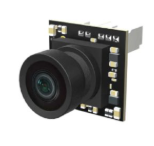
\includegraphics[width=1\linewidth]{fpvcam.png}
          \caption{Caddx Ant Lit Analog Camera}
          \label{fig:fpvcam}
        \end{wrapfigure}

        This FPV cam is good for the following reasons:
        \begin{itemize}
          \item \textbf{\textit{Ultra-Low Latency Analog Transmission:}} The Ant Lite supports analog video out, which is preferred in FPV racing and manual drone piloting due to its near-zero latency — crucial for split-second control.
          \item \textbf{\textit{1200TVL Resolution:}} Offers high clarity and detail with 1200TVL (TV lines), ensuring pilots can clearly identify obstacles, gates, and terrain features during flight.
          \item \textbf{\textit{Wide Field of View (FOV):}} Features a 2.1mm lens with a wide FOV (up to 165°), giving the pilot a broad visual perspective, which enhances situational awareness and spatial navigation.
        \end{itemize}
        \clearpage
        \subsubsection{\large Transmitter}
        \begin{wrapfigure}{r}{0.3\textwidth}
          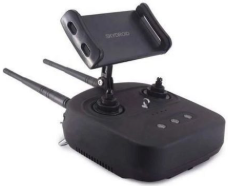
\includegraphics[width=1\linewidth]{transmitter.png}
          \caption{Radiomaster Pocket Radio CC2500/ELRS}
          \label{fig:transmitter}
        \end{wrapfigure}
        Reasons why we chose this transmitter:
        \begin{itemize}
          \item \textbf{\textit{Multiprotocol Support (CC2500 Variant):}} It supports many popular protocols: FrSky D8/D16, Futaba SFHSS, Radiolink, etc.
          \item \textbf{\textit{ELRS 2.4GHz: Ultra-Responsive \& Long-Range:}} We're using ELRS protocol and this transmitter supports that. ELRS allows low-latency and long-range commuincation which is ideal for our use case.
          \item \textbf{\textit{OpenTX/EdgeTX Firmware:}} Runs EdgeTX, a customizable, open-source firmware for transmitters. Lets us configure \textbf{custom mizes, telemetry screens, voice alerts, programmable switches.}
          \item \textbf{\textit{Telemetry Support:}} When paired with the RP1 V2 or telemetry-capable CC2500 receivers, it supports real-time telemetry data: \textit{battery voltage, GPS coordinates, RSSI, link quality etc.}
        \end{itemize}

        \textcolor{red}{\textbf{Problem:} we're using mavlink and elrs.. but that is not compatible.. we need to discuss and clarify this part.}

    \section{Autonomous Navigation System}
      \subsection{Hardware Setup}
      The hardware setup for autonomous navigation primarily consists of -
      \begin{enumerate}
        \item M8N GPS sensor with Magnetometer.
        \item 8X 360 degree ultrasonic sensor array for proximity sensing (collision avoidance).
        \item Front-facing camera sensor for scene detection (collision avoidance).
        \item Down-facing camera sensor for identifying the landing pad.
        \item Pixhawk 2.4.8 Flight Controller for UAV control after issuance from flight computer.
        \item Jetson Nano (onboard flight computer) for mission execution and path planning.
      \end{enumerate}
      \subsection{Software Architechture}
      The software setup for autonomous navigation primarily consists of - 
      \begin{enumerate}
        \item ROS2 for providing the inter-nodal communication during operation.
        \item Ardupilot MissionPlanner GCS for geofencing and manual/autonomous operation control.
        \item Tensorflow based custom trained Neural Network for disaster identification.
        \item OpenCV for "stiching the frames" from the downward feed to obtain a collective map of the area for more accurate counting.
        \item Marker Tracker library for autonomous payload dropping.
        \item Failsafe ROS2 node which stops the UAV in 3d space in order to a prevent collision by utilizing data from the Ultrasonic Sensor Array.
      \end{enumerate}


    \section{C.G. Calculation \& Stability Analysis}
      \subsection{Lift, Drag and Stability Considerations}
      \subsection{Center of Gravity Position \& Trim}

  % =========== Computationl Analysis ============
  \chapter{Computational Analysis}
    \section{CFD / FEM / MATLAB Simulations}
    \subsubsection{\large CFD Analysis}
    The airflow around the drone was analyzed to optimize lift, minimize drag, and improve stability during low-speed operations like payload drop and hovering. Simulations focused on propeller wash interactions, pressure distribution, and vortex formation near the arms. This helped in validating the positioning of rotors and the overall aerodynamics of the UAV.

    \subsubsection{\large FEM Analysis}
    FEM simulations were analyzed on the frame and arm structures to assess stress concentration under typical flight loads and possible deformations. The goal was to verify that the ABS frame would withstand static and dynamic loads without deformation or failure. Stress, strain, and displacement plots were generated to ensure safety margins under thrust and payload weight.\\

Open-source and proprietary tools like ANSYS and SolidWorks Simulation were used. These analyses guided material thickness choices, arm length adjustments, and center of mass alignment to enhance both flight performance and structural durability.



    \section{CAD Model and Performance Validation}
    A comprehensive 3D CAD model of the drone was created using SolidWorks to visualize and validate all mechanical subsystems.
    \begin{enumerate}
      \item \textbf{Spatial Layout:} The CAD model ensured that all components — motors, ESCs, battery, payload, flight controller, and camera — were properly mounted without interference. Special attention was given to propeller clearance, wiring space, and CG alignment.
      \item \textbf{Mass and Balance Validation:} Using the CAD tool’s mass properties feature, it is confirmed the total takeoff weight and ensured that the center of gravity (CG) fell within the desired range for stable flight. 
      \item \textbf{Design-to-Prototype Transition:} The finalized CAD was used to generate 2D technical drawings for 3D printing, and component fabrication. It served as the backbone for building a physically accurate prototype, ensuring minimal mismatch between design and build.
    \end{enumerate}
  % =========== Safety, Compliance & Risk Assessment====== 
  \chapter{Safety \& SORA Assessment}
    \subsubsection{\Large Risk Analysis and Mitigation Strategies}
      
  % ========= Conclusion & Future Work =====
  \chapter{Methodology for Autonomous Operations}
    \section{Flight Control Algorithm}
    The flight control algorithm primarily consists of a setup based upon the ROS2 architecture. Here, multiple operation nodes will be executed as subroutines based upon their required use. The communication between the nodes will be based upon a subscriber-publisher relationship.\\

Under the various nodes, there is a primary node which decides upon the flight path. The flight path is generated using the geofence co-ordinates as the boundary then a maximum coverage algorithm is utilised to effectively scan the whole bound area for objects and disaster scenarios. The master node also runs the image recognition model which identifies objects in the frame. Then a counter slave node is called upon which inputs the incoming feed and outputs the number of objects identified under each class. This is a separate CNN meant for accurate counting. Another slave node is present for more classification of the disaster once a signal is received from the master node. The type of disaster is returned to the master node. The same feed is sent into a "headcount" which identifies the number for human bodies in the frame to look for potential survivors in the area, after notification from the master node.\\

As the mapping is completed, a "stiching" node inputs the video feed to turn the feed into a panorama map by utilizing the time series accelerometer data. This is then further fed into the object classification node for a final object count to ensure optimal accuracy. The following routine is executed during the Autonomous operation of the UAV. Our unique approach to cross checking with the stiched map ensures accuracy as it directly reduces the chances for one object getting counted multiple times if the UAV crosses an area twice. The divided processing approach based on the nodal architecture ensures optimal computation usage and saves on energy as well, which is an important factor for on-board processing systems.

    \section{Object Detection \& Counting}
    \section{Autonomous Payload Drop Mechanism (Gripper)}

  \chapter{Innovations and Future Scope}
  \chapter{Bill of Materials}
    \begin{table}[h!]
      \centering
      \caption{Bill of Materials} \vspace{0.2cm}
        \begin{tabular}{|l|c|c|}
          \hline
          \textbf{Component Name} & \textbf{Quantity} & \textbf{Unit Price {INR}} \\
          \hline
          NVIDIA Jetson Orin Nano 8GB & 1 & 36,499 \\
          Pixhawk 2.4.8 Flight Controller & 1 & 11,179 \\
          Cameras & 2 & 1,000 \\
          SpeedyBee BL32 50A 4-in-1 ESC &1 &7139\\
          DYS D2836-7 1120KV Brushless Motor &4 &1,228\\
          Orange Pro-Range 5200mah 11.1V & 1 &3,653\\
          GPS – Neo M8N  &1 &1,500\\
          SkyDroid Transmitter  &1 & 12,075\\
          Servo & 1& 500\\
          Frame  &1& 3,000\\
          9-inch Propellers & 4 &200\\
          \hline
          \textbf{Total}  & --  & \textbf{83,257 /-}   \\      
          \hline
        \end{tabular}
    \end{table}

   \chapter{Appendix} 

\end{document}

